\documentclass[10pt,aspectratio=169]{beamer}
\usetheme[progressbar=frametitle]{metropolis}
\usepackage{booktabs}
\usepackage{amsmath}
\graphicspath{{../output/}}
\setbeamertemplate{frame numbering}[fraction]

\title{Replicating Abadie, Diamond \& Hainmueller (2010)}
\subtitle{Synthetic control and California's Proposition 99}
\author{Qiaoshi Yang}
\institute{STAT 5200: Applied Econometrics \quad Replication presentation}
\date{November 2026}

\begin{document}

\maketitle

%----------------------------------------------------------------------
\begin{frame}{The paper and why I chose it}
\textbf{Abadie, Diamond \& Hainmueller (2010)}, \emph{JASA} 105(490): 493--505.

\medskip
\textbf{Question.} What happened to cigarette sales in California because of
Proposition 99, a 1988 tobacco control program?

\medskip
\textbf{Why it is hard.} One treated state. No other state looks like
California before 1988, so a simple DiD against ``the rest of the US'' is not
credible.

\medskip
\textbf{Contribution.} The synthetic control method: build the comparison
unit as a data-driven weighted average of untreated states, and do inference
by placebo permutation.

\medskip
\textbf{Link to my project.} Massachusetts passed an almost identical
program in 1992 (Question 1). My project applies the same design, data and
code to Massachusetts and compares it with DiD and synthetic DiD.
\end{frame}

%----------------------------------------------------------------------
\begin{frame}{Setting: Proposition 99}
\begin{columns}[T]
\begin{column}{0.42\textwidth}
\begin{itemize}
\item Passed November 1988, in effect January 1989
\item Cigarette excise tax $+25$ cents per pack
\item Revenue earmarked for health and anti-smoking education: media
campaigns, school programs, local clean-air ordinances
\item Over \$100 million per year in anti-tobacco projects at first
\end{itemize}
\end{column}
\begin{column}{0.56\textwidth}
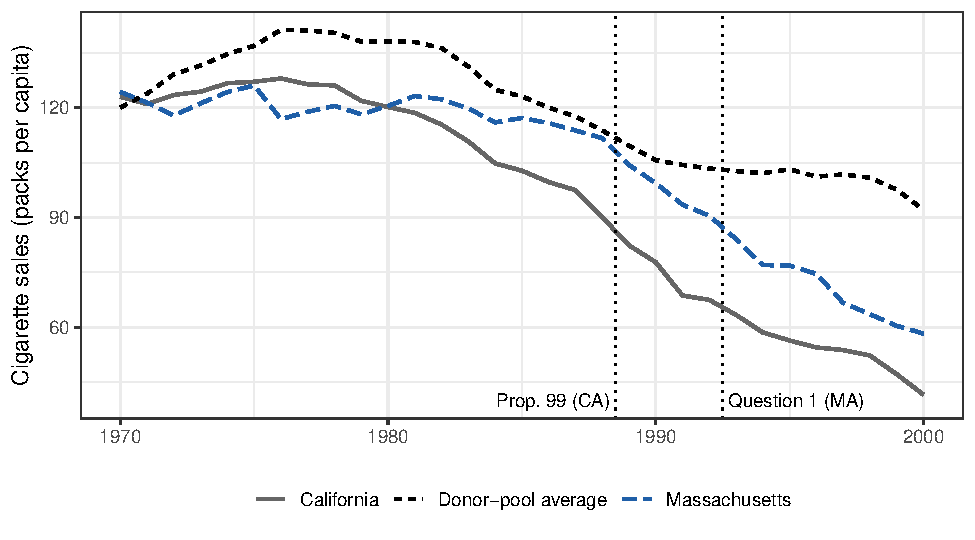
\includegraphics[width=\linewidth]{trends.pdf}

{\footnotesize Per-capita sales. California was already declining faster than
the donor average before 1989.}
\end{column}
\end{columns}
\end{frame}

%----------------------------------------------------------------------
\begin{frame}{Method: synthetic control}
States $j = 1$ (California) and $j = 2,\dots,J+1$ ($J = 38$ donors); last
untreated year $T_0 = 1988$. The effect in year $t > T_0$ is
\[
  \alpha_{1t} = Y_{1t}^{I} - Y_{1t}^{N}, \qquad
  \hat Y_{1t}^{N} = \sum_{j=2}^{J+1} w_j^{*} Y_{jt}, \quad
  w_j \ge 0,\ \sum_j w_j = 1 .
\]
Weights match pre-1989 predictors $X_1$ (California) and $X_0$ (donors):
\[
  W^{*}(V) = \arg\min_{W}\ (X_1 - X_0 W)' V (X_1 - X_0 W),
\]
with diagonal $V$ chosen to minimise the pre-1989 MSPE of sales.

\medskip
\textbf{Why it works.} If sales follow a factor model, matching a long
pre-period of outcomes also matches the unobserved factor loadings. Weights
are non-negative and sum to one, so there is no extrapolation.

\medskip
\textbf{Inference.} Reassign treatment to each donor in turn. Rank
California's post/pre MSPE ratio among all 39 states.
\end{frame}

%----------------------------------------------------------------------
\begin{frame}{Data and design choices in the paper}
\begin{itemize}
\item \textbf{Outcome:} per-capita cigarette sales in packs, 1970--2000,
from tax revenue (Orzechowski \& Walker, \emph{The Tax Burden on Tobacco})
\item \textbf{Predictors:} log income per capita, retail price, share aged
15--24 (averaged 1980--88); beer per capita (1984--88); sales in 1975, 1980
and 1988
\item \textbf{Donor pool, 38 states.} Dropped:
  \begin{itemize}
  \item states with large tobacco programs in 1989--2000: MA, AZ, OR, FL
  \item states that raised cigarette taxes by 50 cents or more: AK, HI, MD,
  MI, NJ, NY, WA
  \item District of Columbia
  \end{itemize}
\item \textbf{Sample ends in 2000}: after that many states adopted
anti-tobacco measures (e.g.\ the 1998 Master Settlement Agreement)
\end{itemize}
\end{frame}

%----------------------------------------------------------------------
\begin{frame}{Paper's results}
\begin{itemize}
\item Synthetic California = Utah 0.334, Nevada 0.234, Montana 0.199,
Colorado 0.164, Connecticut 0.069
\item Pre-1989 fit is close: MSPE about 3
\item By 2000, sales were \textbf{about 26 packs per capita lower} than
synthetic California
\item Average over 1989--2000: almost 20 packs lower, \textbf{about 25\%}
\item California's post/pre MSPE ratio is about 130, the largest of the 39
states: \textbf{permutation $p = 1/39 = 0.026$}
\end{itemize}
\end{frame}

%----------------------------------------------------------------------
\begin{frame}{My replication}
\textbf{Goal:} rebuild the data from public sources and reproduce the
analysis with the original estimator, not with the authors' data file.

\medskip
\begin{tabular}{@{}ll@{}}
\toprule
Ingredient & Source used here \\
\midrule
Sales and price & CDC STATE System, \emph{Tax Burden on Tobacco 1970--2019} \\
Income & BEA SAINC1, per capita personal income (nominal, logged) \\
Share aged 15--24 & NCI SEER population by age \\
Beer & NIAAA apparent consumption, gallons per resident 14+ \\
Estimator & R package \texttt{Synth} (same as the authors' software) \\
\bottomrule
\end{tabular}

\medskip
\begin{itemize}
\item Same donor pool, same predictors and averaging windows
\item Pipeline: \texttt{Rscript run\_all.R} downloads the raw data and
regenerates every table and figure
\item Code: \url{https://github.com/yang-qs/stat5200-project}
\end{itemize}
\end{frame}

%----------------------------------------------------------------------
\begin{frame}{Predictor balance: paper vs replication}
\centering
\begin{tabular}{lcccc}
\toprule
 & \multicolumn{2}{c}{ADH (2010)} & \multicolumn{2}{c}{Replication} \\
\cmidrule(lr){2-3}\cmidrule(lr){4-5}
 & California & Synthetic & California & Synthetic \\
\midrule
Ln(income per capita) & 10.08 & 9.86 & 9.65 & 9.49 \\
Retail price & 89.42 & 89.41 & 96.57 & 97.97 \\
Share aged 15--24 (\%) & 17.40 & 17.40 & 17.32 & 17.04 \\
Beer per capita (gal.) & 24.28 & 24.20 & 29.79 & 30.03 \\
Packs per capita, 1975 & 127.10 & 126.99 & 127.10 & 126.73 \\
Packs per capita, 1980 & 120.20 & 120.43 & 120.20 & 120.44 \\
Packs per capita, 1988 & 90.10 & 91.62 & 90.10 & 92.11 \\
\bottomrule
\end{tabular}


\medskip
\begin{minipage}{0.85\textwidth}\footnotesize
Prices in cents. Lagged sales match the paper to the decimal. Covariate
levels differ because the definitions differ: nominal personal income
vs.\ 1997 dollars, beer per resident 14+ vs.\ per capita, a revised price
series. Each state's predictors use the same definition, so only relative
positions matter for the weights.
\end{minipage}
\end{frame}

%----------------------------------------------------------------------
\begin{frame}{Synthetic California: weights and paths}
\begin{columns}[T]
\begin{column}{0.34\textwidth}
\centering
\resizebox{\linewidth}{!}{\begin{tabular}{lcc}
\toprule
State & ADH (2010) & Replication \\
\midrule
UT & 0.334 & 0.367 \\
CO & 0.164 & 0.316 \\
NV & 0.234 & 0.237 \\
MT & 0.199 & -- \\
CT & 0.069 & 0.077 \\
\bottomrule
\end{tabular}
}

\medskip
{\footnotesize Four of the paper's five donors come back. Montana drops
out and Colorado's weight roughly doubles.}
\end{column}
\begin{column}{0.63\textwidth}
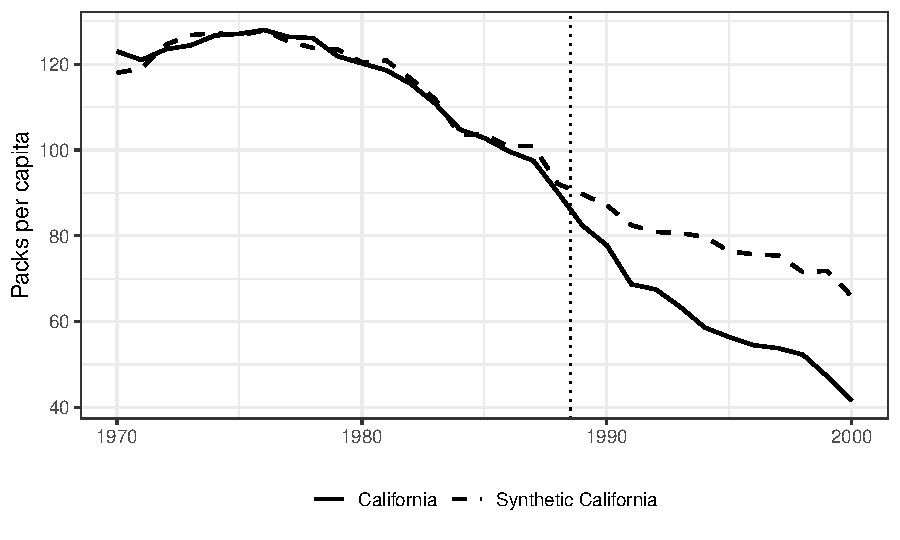
\includegraphics[width=\linewidth]{ca_path.pdf}
\end{column}
\end{columns}
\end{frame}

%----------------------------------------------------------------------
\begin{frame}{Inference: placebos in space}
\begin{columns}[T]
\begin{column}{0.49\textwidth}
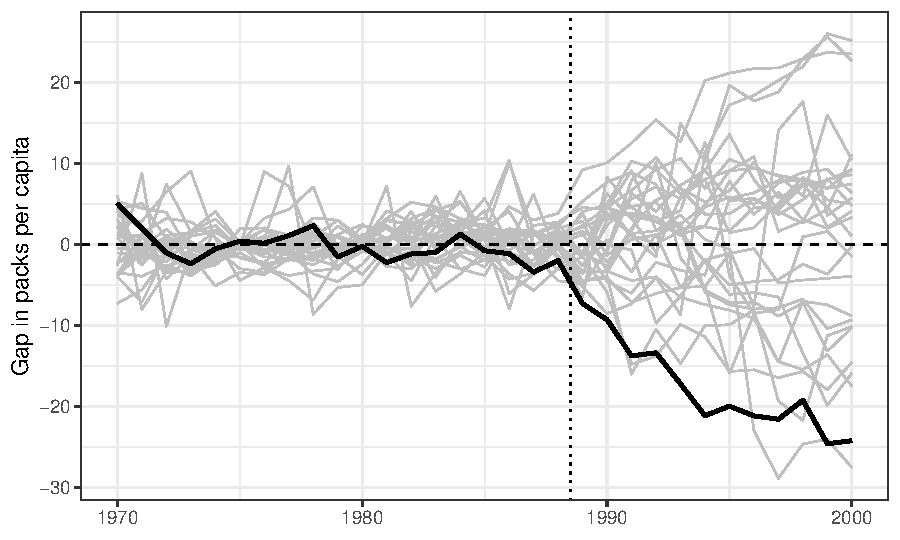
\includegraphics[width=\linewidth]{ca_placebo.pdf}

{\footnotesize Gaps for California (black) and the placebo states (grey).
Placebos with pre-1989 MSPE above 5 times California's are dropped, as in
the paper's Figure 6.}
\end{column}
\begin{column}{0.49\textwidth}
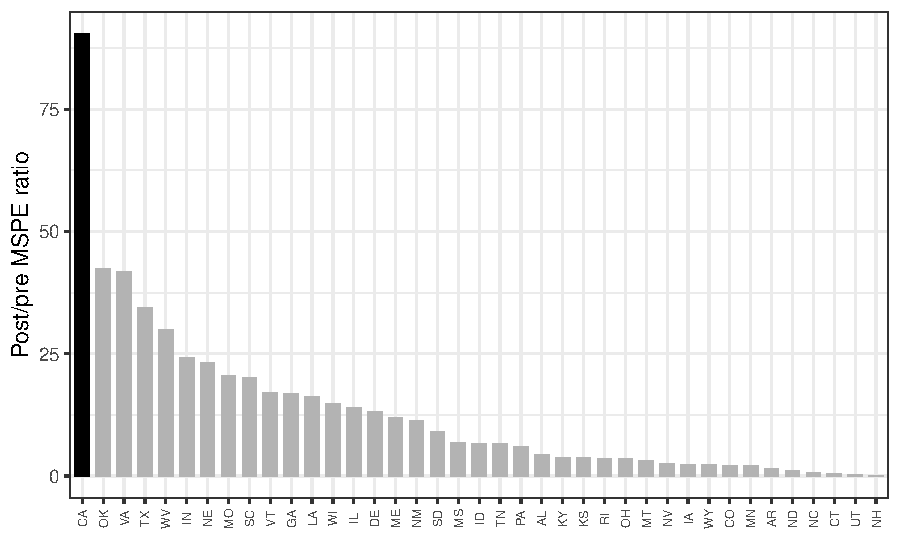
\includegraphics[width=\linewidth]{ca_ratio.pdf}

{\footnotesize Post/pre MSPE ratio (cf.\ paper's Figure 8). California
ranks first of 39.}
\end{column}
\end{columns}
\end{frame}

%----------------------------------------------------------------------
\begin{frame}{Headline numbers}
\centering
\begin{tabular}{lcc}
\toprule
 & ADH (2010) & Replication \\
\midrule
Pre-1989 MSPE & about 3 & 3.8 \\
Gap in 2000 (packs) & about $-26$ & $-24.3$ \\
Average gap 1989--2000 (packs) & almost $-20$ & $-17.8$ \\
Average gap, \% of synthetic & about $-25$\% & $-23$\% \\
Post/pre MSPE ratio & about 130 & 90 \\
Rank of California among 39 & 1 & 1 \\
Permutation $p$-value & $1/39 = 0.026$ & $0.026$ \\
\bottomrule
\end{tabular}


\medskip
\begin{minipage}{0.8\textwidth}
The qualitative result and the inference replicate exactly. The point
estimate is about 10\% smaller, and the fit is a bit worse, so the MSPE
ratio is lower. The $p$-value is identical because California still has the
largest ratio.
\end{minipage}
\end{frame}

%----------------------------------------------------------------------
\begin{frame}{Lessons from the replication}
\begin{enumerate}
\item \textbf{Data vintage matters, but less than I expected.} Lagged sales
match the paper exactly, while the price series and every covariate differ
in definition or source. The 2000 gap moved by about 2 packs.
\item \textbf{Read the paper closely.} Table 1 says ``Ln(GDP per capita)'' in
1997 dollars; the text and data appendix say log personal income. I followed
the appendix.
\item \textbf{Weights are less stable than the counterfactual.} Small data
changes dropped Montana and doubled Colorado, but the synthetic path and the
gap barely moved. Interpret the path, not individual weights.
\item \textbf{Software is fragile.} \texttt{Synth}'s optimizer failed on one
placebo state in the Massachusetts design; I added a retry with looser
tolerances.
\item \textbf{Fiscal vs.\ calendar years.} Sales are by fiscal year (ending
June 30). Following the paper, the fiscal year containing the January tax
increase is the first treated year.
\end{enumerate}
\end{frame}

%----------------------------------------------------------------------
\begin{frame}{How this informs my project: Massachusetts 1992}
\begin{columns}[T]
\begin{column}{0.48\textwidth}
\begin{itemize}
\item Question 1: tax $26 \to 51$ cents on 1 January 1993, revenue funds a
tobacco control program
\item Same data, donor pool, predictors and code as the replication, so
differences in answers are not differences in method
\item Synthetic MA = CT 0.49, DE 0.29, UT 0.15, RI 0.07
\item Average gap 1993--2000: $-18.5$ packs (21\%); permutation $p = 0.077$
\item Add TWFE DiD and synthetic DiD (Arkhangelsky et al.\ 2021) to see how
much the estimator matters
\end{itemize}
\end{column}
\begin{column}{0.50\textwidth}
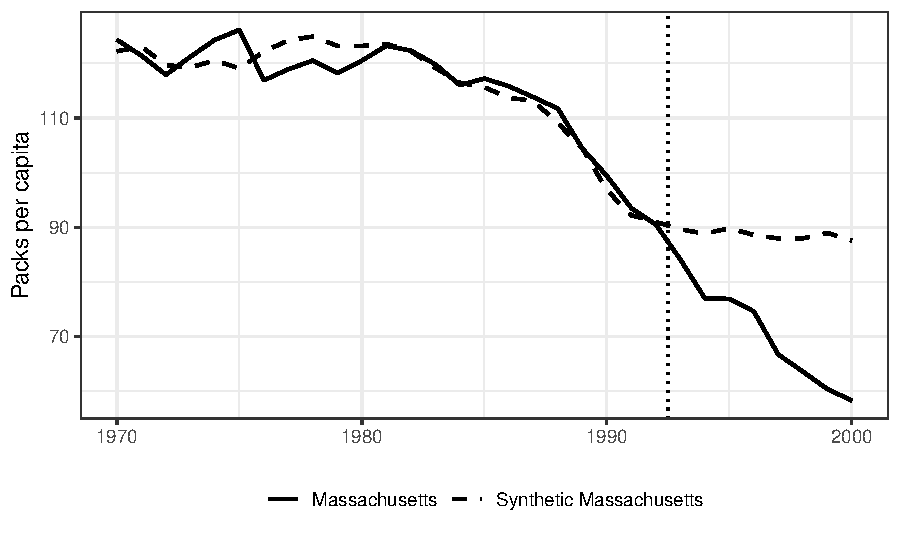
\includegraphics[width=\linewidth]{ma_path.pdf}
\end{column}
\end{columns}
\end{frame}

%----------------------------------------------------------------------
\begin{frame}{Takeaways}
\begin{itemize}
\item The main result of ADH (2010) replicates from public data: a gap of
24 packs by 2000 (paper: 26), and California ranks first of 39 placebos
($p = 0.026$).
\item The method is transparent about its comparison unit: the weights and
pre-period fit can be inspected and criticised.
\item With one treated unit, inference rests on placebo permutations, and the
smallest attainable $p$-value is $1/(J+1)$.
\item Open issues the paper shares with my project: sales are not smoking
(cross-border purchases), and the treatment bundles a tax with a program.
\end{itemize}

\vfill
\centering Thank you. \quad Code: \url{https://github.com/yang-qs/stat5200-project}
\end{frame}

%----------------------------------------------------------------------
\appendix
\begin{frame}{References}
\footnotesize
Abadie, A., Diamond, A., and Hainmueller, J. (2010). Synthetic control methods
for comparative case studies: Estimating the effect of California's tobacco
control program. \emph{Journal of the American Statistical Association},
105(490):493--505.

\medskip
Abadie, A. and Gardeazabal, J. (2003). The economic costs of conflict: A case
study of the Basque Country. \emph{American Economic Review}, 93(1):113--132.

\medskip
Arkhangelsky, D., Athey, S., Hirshberg, D.~A., Imbens, G.~W., and Wager, S.
(2021). Synthetic difference-in-differences. \emph{American Economic Review},
111(12):4088--4118.

\medskip
Orzechowski and Walker (2019). \emph{The Tax Burden on Tobacco, 1970--2019}.
CDC STATE System, dataset \texttt{7nwe-3aj9}.
\end{frame}

\end{document}
